\chapter{Difficultés rencontrées}

Un certain nombre de problèmes ont été rencontrés tout au long du développement
du projet. Ces complications sont de nature technique (par exemple avec la mise
en place du GUI, la gestion de l'alpha avec les textures) mais principalement de
nature géométrique.

\section{Notations matricielles américaine et française}

Le premier problème, qui a apporté un certain sentiment de confusion, a été le
sens de notation. En effet, les notations américaine et française pour
l'écriture matricielle ne sont pas les mêmes. Les colonnes et les lignes sont
inversées entre les deux.\\

Comme il a été décidé de ne pas reprendre le framework fourni dans les TPs, mais
de réécrire complétement une plateforme from scratch, tous les calculs pour des 
classes de base (\emph{Matrix4}, \emph{Vec3}, etc...) ont été réalisés en utilisant la
notation matricielle française. Cependant, le système de la caméra libre a été
conçu d'après le TP concerné et plusieurs ressources sur Internet. Il y a donc
eu une confusion sur l'écriture, puisque la totalité des ressources consultées 
concernaient la notation américaine. Ainsi, une quantité importante de soucis
liés à ces malentendus est apparue, principalement pour la gestion des
transformations de la camera, et le calcul de la matrice \emph{MVP}. Par exemple, une
déformation importante de l'objet était présente, comme sur une caméra avec un
objectif de type FishEye. Mais le but étant d'obtenir une caméra classique,
l'ensemble des matrices a été uniformisé dans la notation française.

\section{Rotation semi-automatique de la caméra}

\section{Gestion de l'alpha des textures}

Les particules sont toutes considérées comme un point unique de l'espace, sur
lesquelles est appliquée une texture. Dans un premier temps, la texture était un
simple carré blanc. Puis celle-ci a évolué pour une image plus complexe,
comportant un canal alpha.

\begin{figure}[h]
	\begin{center}
		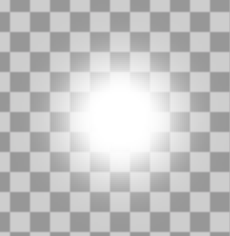
\includegraphics[width=0.2\textwidth]{img/33-texture.png}
	\end{center}
	\caption{Texture avec présence du canal alpha}
\end{figure}

Par défaut, OpenGL ne reconnaît aucun canal alpha avec les textures. Il faut le
préciser à l'aide des constantes spécifiques. Le chargement de la texture se
fait à travers la classe \emph{Texture}. Dans un premier temps, il a été convenu
d'utiliser la fonction \emph{glBlendFunc} avec différentes constantes, comme
\emph{GL\_SRC\_ALPHA}. Cependant cette fonction n'a pas convenu à l'usage ci-présent,
car elle d'une part beaucoup plus utilisée pour la gestion des couleurs
directement en OpenGL, et d'autre part la texture n'est pas appliquée sur une 
zone spécifique, mais sur un point.\\

C'est dans la fonction \emph{glTexImage2D} qu'il faut s'orienter. Celle-ci possède
notamment un paramètre permettant de définir le nombre de couleurs composant
l'image à utiliser en texture. La constante \emph{GL\_RGBA} est à associer à cette
fonction, et permet ainsi un gestion du canal alpha pour cette texture de
particule.

\section{Insertion du rendu OpenGL dans un GUI}

Une des consignes du projet était d'avoir une interface Qt autour de la fenêtre
de rendu OpenGL. Cette interface doit permettre, au travers de boutons ou autres
éléments d'interface, de changer plusieurs paramètres de l'émetteur mis en
place. Personne ne possédant d'expérience avec les GUI et Widget Qt, un
apprentissage en plus a dû être réalisé. Dans un premier temps, une fenêtre Qt 
de type « MainWindow » a été utilisé. Pour des raisons qui sont toujours
obscures (il s'agirait sans doute d'un problème lié à la plateforme Mac OSX), il
est impossible de dessiner le rendu OpenGL. Un message indique que la taille du
widget contenant le rendu est trop petite, même pour une taille dix fois plus
grande que le rendu.\\

La solution est d'avoir une base simple, c'est à dire un simple Widget Qt en
fenêtre principale. Il suffit d'adapter par la suite l'application existante
pour l'inclure dans ce nouveau widget, puis de réaliser les \emph{bind}
nécessaires pour relier les actions des boutons de l'interface aux actions de
l'application. Il ne faut également pas oublier de déplacer la prise en compte
des évènements claviers dans le widget parent, mais pas nécessairement les
évènements souris.
